\documentclass[twocolumn,aps,prb,citeautoscript]{revtex4-1}
\usepackage{graphicx,amsmath,amssymb,subcaption,tabularx,array}

\begin{document}

\newcolumntype{R}[1]{>{\raggedleft\arraybackslash}p{#1}}

\title{Effects of a superconducting lead endcap \\ on the magnetic field
profile for the nEDM search}
\author{Aritra Biswas, with Filippone Group}
\affiliation{Kellogg Radiation
Laboratory, California Institute of Technology}

\begin{abstract}
Discovery of a non-zero electric dipole moment in the neutron (nEDM) would indicate a CP violation,
with implications for
extending the Standard Model and confirming predictions about matter-antimatter asymmetry.
Experiments using shifts in neutron
precession frequency to measure the nEDM require a uniform magnetic field to prevent false signals.
We investigate the
effectiveness of a superconducting lead endcap in promoting field uniformity inside an open-ended cylindrical coil.
Measured field maps in the superconducting state closely match simulations and indicate that the endcap causes field
peaks to shift away from magnet center, decreasing field gradients in desired regions. Simulations also suggest that
the endcap may prevent field effects caused by imperfections in the geometry of an axial lead shield that surrounds
the coil.
\end{abstract}

\maketitle

\section{Motivation}

CP violation plays a critical role in explaining matter-antimatter asymmetry in the universe and
guiding
theories beyond the Standard Model; as such, the search for instances of CP violation is 
ongoing \cite{cpv,ill}.
A non-zero electric dipole moment (EDM) in the neutron would constitute such a violation and can be measured
through the shift in Larmor precession frequency of neutrons in $\vec{E}$ and $\vec{B}$ fields \cite{pendlebury}.
An experimental limit of $|d_n| < 2.9 \times 10^{-26}\;e\cdot\text{cm}$ was established by ILL in 2006\cite{ill}.

Experiments using these methods are prone to a geometric phase (GP) effect, caused by gradients of the $\vec{B}$
field, that can lead to a false signal, i.e. the measurement of a non-zero EDM even if the real EDM is zero.
\cite{ill,pendlebury}. As part of an effort to improve the measured limit, we have construced a half-scale model of
a neutron EDM (nEDM) measurement experiment,
using new methods to minimize errors such as the GP effect. Preventing the GP
requires precise engineering to create a space-uniform magnetic field. To accomplish this, 
we use a coil tuned to create an uniform magnetic field, surrounded by
shielding made of ferromagnetic Metglas and superconducting lead.

Here, we introduce a new shielding component - a superconducting lead top endcap - into the half-scale model. We
compare its effects on the magnetic field to simulations, predict its effect on field gradients in the volumes in
which neutrons will travel in the full-scale nEDM experiment, and analyze the desirability of including a similar
endcap in the full-scale experiment.

\section{Introduction \\ to the half-scale model}

At the center of the half-scale model (magnet center)
are two fiducial 3.8 cm $\times$ 5 cm $\times$ 20 cm volumes.
In the full-scale experiment, these volumes will be the measurement cells in which
precession measurements of trapped ultra-cold neutrons (UCN) will take
place, so the goal is to achieve field uniformity within.

\begin{figure}
    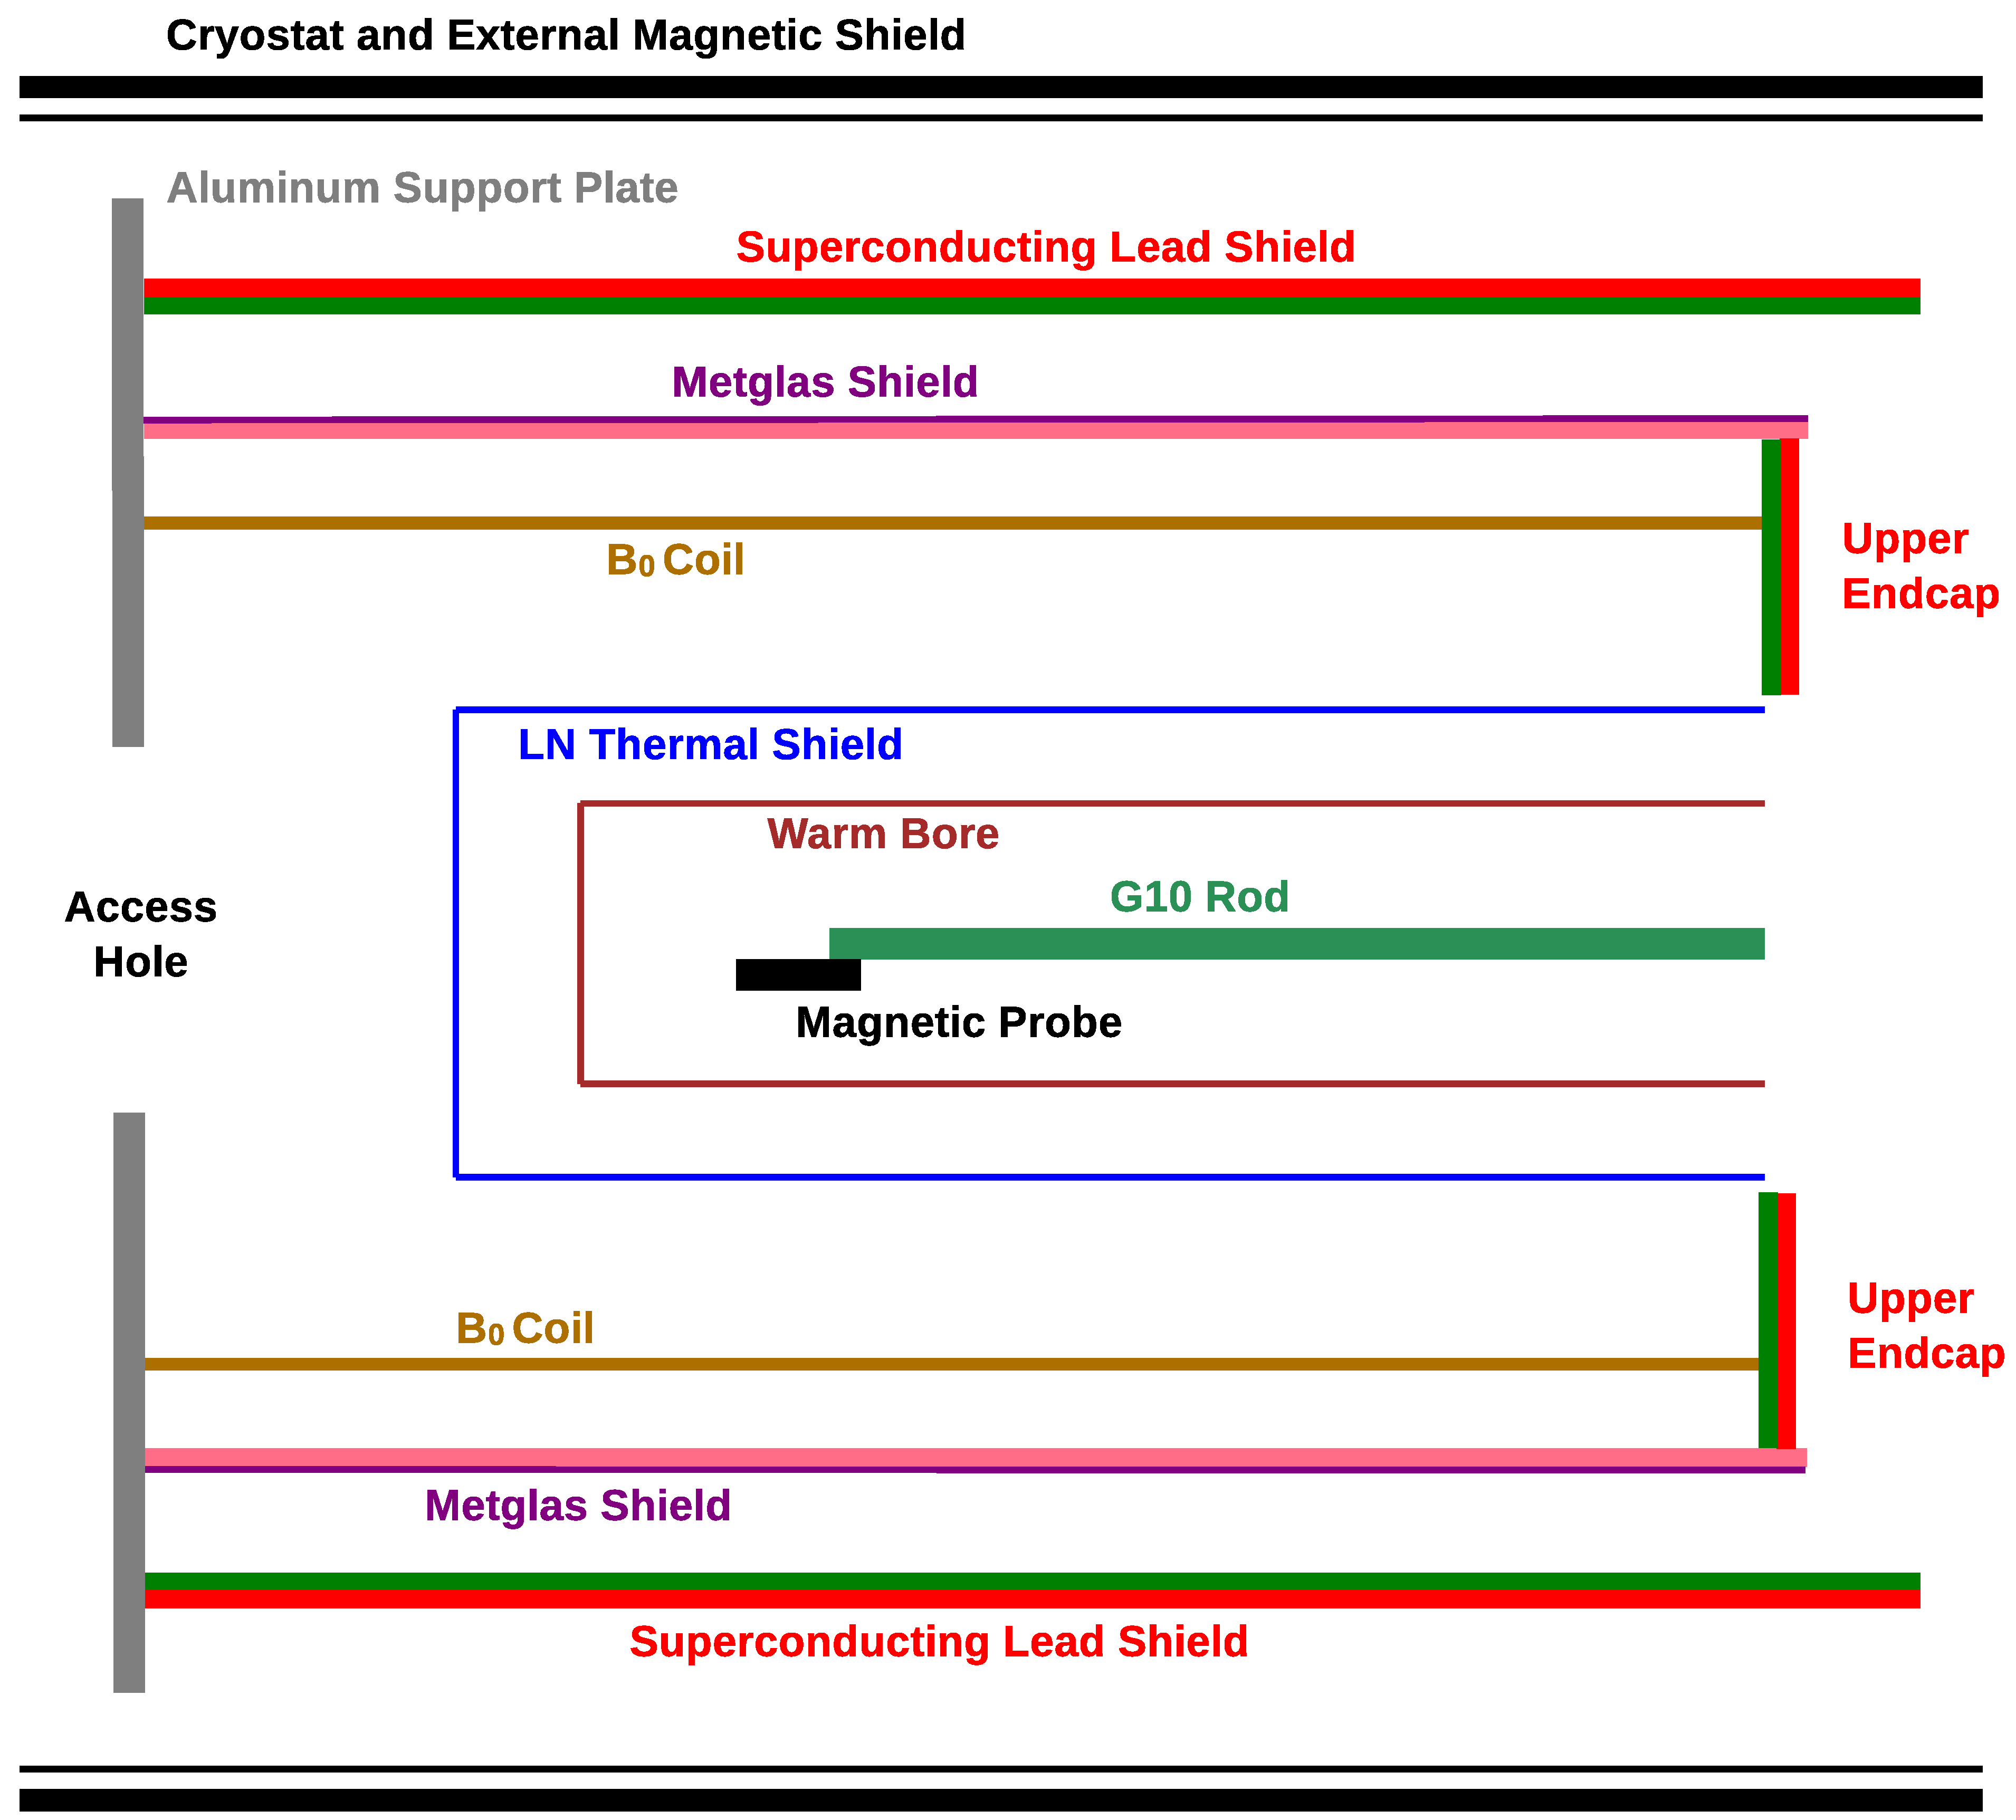
\includegraphics[angle=90, width=0.45\textwidth]{figures/structure.eps}
    \caption{\label{fig:structure}Stylized diagram of the half-scale model, showing a vertical
    cross-section of the cylindrical apparatus. The vertically-oriented layers shown above
    - i.e. the cryostat shield, lead shield, Metglas shield, coil, thermal shield, and warm bore -
    are concentric cylinders nested inside one another.
    The G10 rod is shown along the $z$-axis: the common central axis of the cylinders. The endcap
    sits on top.}
\end{figure}

The magnetic field is generated by the $B_0$ coil, a cylindrical structure with wires along its
surface in a $\cos\theta$ coil geometry that creates a magnetic field orthogonal to the cylinder's
central axis\cite{coil}. Concentric cylindrical shielding structures (shown in Figure \ref{fig:structure})
surround the $B_0$ coil; cylinders are nested one inside the other in a structure resembling ``Russian dolls.''

We define the $z$-axis as the common central axis of these cylinders, and the $x$-axis as the primary direction
of the magnetic field.

The $B_0$ coil, of course, cannot create a sufficiently uniform field without the surrounding shielding.
The ferromagnetic Metglas shield redirects the field and promotes uniformity near magnet center. The cylindrical
superconducting lead shield (axial shield) protects the field from environmental gradients and fluctuations.

The lead endcap (the focus of this study) has an annular cross-section and lays on top of the cylindrical
shields. We include it in an attempt to mitigate edge effects of the magnetic field;
expectations of the endcap's behavior are discussed further in the next section.

The whole apparatus is placed inside a cryostat capable of bringing the lead components (the axial shield and
the endcap) to 4 K. A thermal shield and warm bore are placed in the center: the warm bore is kept at room
temperature and contains the magnetic probe.

\section{Expectations of endcap behavior}

Without the endcap, we expect the field near the open ends of the $B_0$ coil to exhibit edge effects similar to
those shown in Figure \ref{fig:sketch_noendcap}. The obvious correction is a
circular endcap covering the open area, but since the center must be left open for access by the
magnetic probe, we used an annular design. Figure \ref{fig:sketch_endcap} shows the expected influence on
the field's edge effects.

Simulations of the half-scale model with \texttt{RotationShield}, a matrix solver developed previously in the
group,\cite{rotshield} offer more precise predictions. Since the desired field points in the $x$ direction and
edge effects push the field in the $z$ direction, examining $B_x$ and $B_z$ as a function of $z$ near the
height of the endcap ($z = 1.128$ m) offers insight into the endcap's effects. It is important to note
that this curve is interesting only away from the central axis, since $B_z = 0$ everywhere along the central
axis; this is apparent in the sketches (Figure \ref{fig:sketches}) and corroborated by simulations.
Figure \ref{fig:Bz_z_sim} compares simulated field maps without and with an endcap along the off-axis line
$x = 0.1 \text{ m}, y = 0$,
showing the expectation that the endcap will shift
the peak in $B_z$ to higher $z$ (away from magnet center as desired).

\begin{figure*}
    \subcaptionbox{\label{fig:sketch_noendcap}}{\includegraphics[width=0.35\textwidth]{figures/field_noendcap.eps}}
    \;\;\;\;\;\;\;\;\;\;\;\;\;\;\;\;\;\;\;\;\;\;\;\;
    \subcaptionbox{\label{fig:sketch_endcap}}{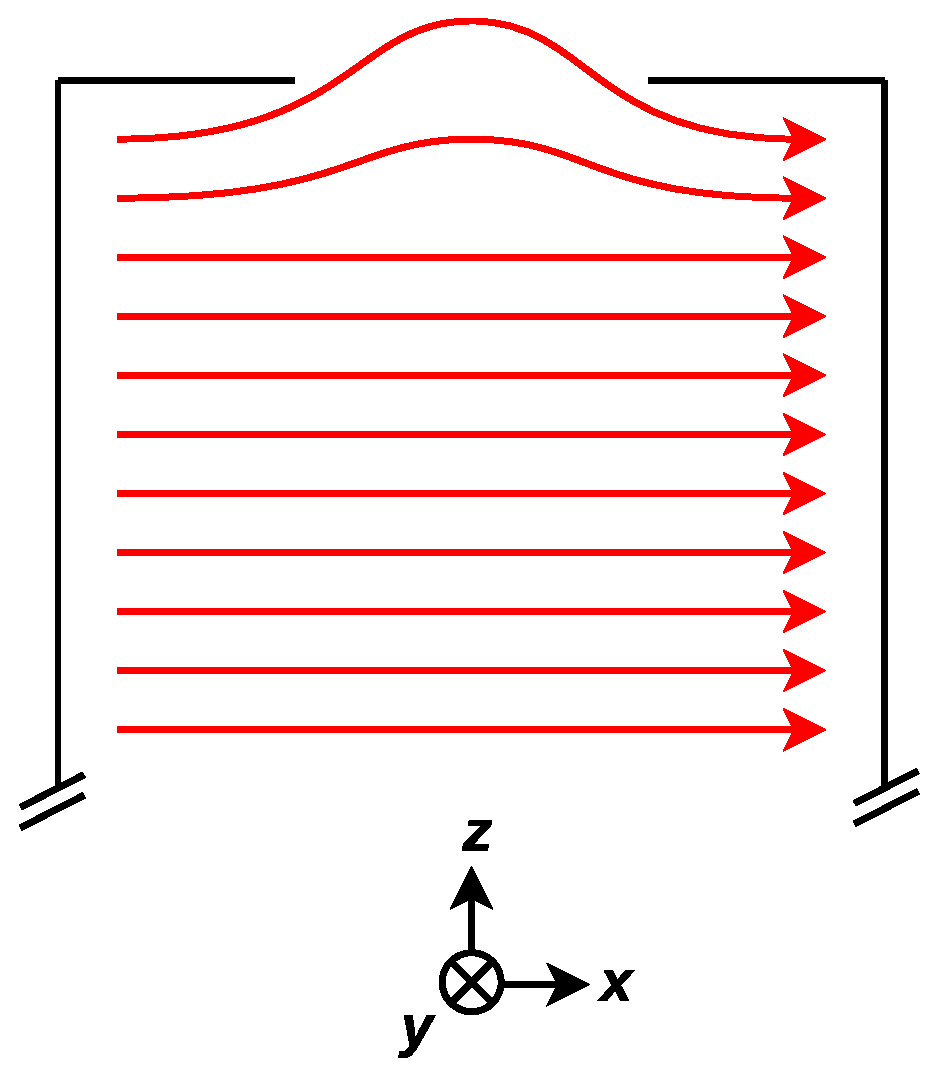
\includegraphics[width=0.35\textwidth]{figures/field_endcap.eps}}
    \caption{\label{fig:sketches} Sketches of the expected magnetic field without (\ref{fig:sketch_noendcap})
    and with (\ref{fig:sketch_endcap}) the endcap. The endcap is expected to mitigate the edge effects and
    point the field more uniformly along the $x$-axis.}
\end{figure*}

\begin{figure*}
    \includegraphics[width=\textwidth]{figures/Bz_z_sim.eps}
    \caption{\label{fig:Bz_z_sim}$B_z$ vs. $z$ as predicted by simulations in two configurations: with the
    superconducting endcap (magenta curve) and without (cyan curve). The axial shield
    is present and superconducting in both curves.}
\end{figure*}

\section{Measurement methods and corrections}

Field maps can be collected by moving the magnetic probe around the warm bore with a 3-axis stepper motor.
We focus on three configurations:
(A) axial shield and endcap in non-superconducting states; (B) axial shield in a superconducting state, endcap
in a normal state; and (C) axial shield and endcap in superconducting states. With selective heating and cooling
of components, we can bring the half-scale model to each of these three configurations.

The resulting field maps, if directly compared to simulations, reveal many discrepancies that result from
measurement errors. Each of these errors, and relevant corrections, are addressed below.

\subsection{Background subtraction}

For each map, we must measure the background magnetic field (i.e. when the $B_0$ coil is turned off) and
subtract this field from the foreground ($B_0$ on). This step allows us to isolate the effects of our changes in
shielding geometry.

\subsection{Probe centering}

We have found that the field profile is highly sensitive to $x$ position. For example, along the cylinder's
central axis ($x=0, y=0$), simulations predict that $B_z$ should be 0; however, when $x\neq0$,
the $B_z$ vs. $z$ curve exhibits
a peak near $z=1.073$ m, the end of the $B_0$ coil. The height of this peak is directly correlated with the $x$
position. Early comparisons showed a $B_z$ vs. $z$ peak even along $x=0, y=0$, and measurements confirmed that
the probe setup is not correctly centered along the $x$ axis. Since such centering is difficult, we measure the
offset and correct for it during data analysis. For example, consider a mapping where the probe is offset by 4 mm
along the positive $x$ direction. Data taken along $x = 0.1$ m, after correction,
is recognized as data taken along $x = 0.104$ m, so we can compare the curve to the appropriate simulated curve.

\subsection{Probe offset}

Our magnetic probe is composed of three separate one-axis probes which are separated along the $z$-axis.
The probe's location corresponds to the location of the $B_z$ probe: the $B_x$ probe is 15 mm above this location,
while the $B_y$ probe is 15 mm below.. Thus when the probe location is read as
$(0, 0, 0)$, the $B_x$ probe, for example, is actually at $(0, 0, 0.015\text{ m})$. The data that we collect
cannot be expressed as a single vector map, then, since we are not guaranteed to have a vector $(B_x, B_y, B_z)$
for every point $(x, y, z)$. In the analysis programs, we implement spatial axes that are
capable of storing an offset vector corresponding to the components
of the field, such that the $z$ axis can be offset depending on whether we are graphing $B_x$ vs. $z$ or
$B_z$ vs. $z$.

\subsection{Probe tilt}

The probe's rigid mount introduces another problem: the probe cannot be perfectly vertical.
Since $B_x >> B_z$ at
magnet center, even a very small angle can make the $B_z$ probe pick up part of the $B_x$ signal;
this effect is illustrated in
Figure \ref{fig:angle}. The probe, tilted at some angle $\theta$, gives skewed readings $B_x'$ and $B_z'$.
The true readings $B_x$ and $B_z$ can be obtained from the skewed readings $B_x'$ and $B_z'$ and the angle
$\theta$ through simple trigonometry.

To determine $\theta$, we observe that in simulations, $B_z = 0$ at magnet center, while measured field maps
show a small nonzero $B_z'$ at magnet center. Assuming that the main source of this error is the probe tilt,
we can estimate the angle $\theta = -\frac{B_z'}{B_x'}$. We consider this a reasonable assumption since
the difference $B_z' - B_z$ seems proportional to $B_x$; this coupling of the components suggests their values
are skewed by the probe angle. Furthermore, we apply this correction last to ensure that probe tilt is the main
remaining source of error.

\begin{figure}
\vspace{15pt}
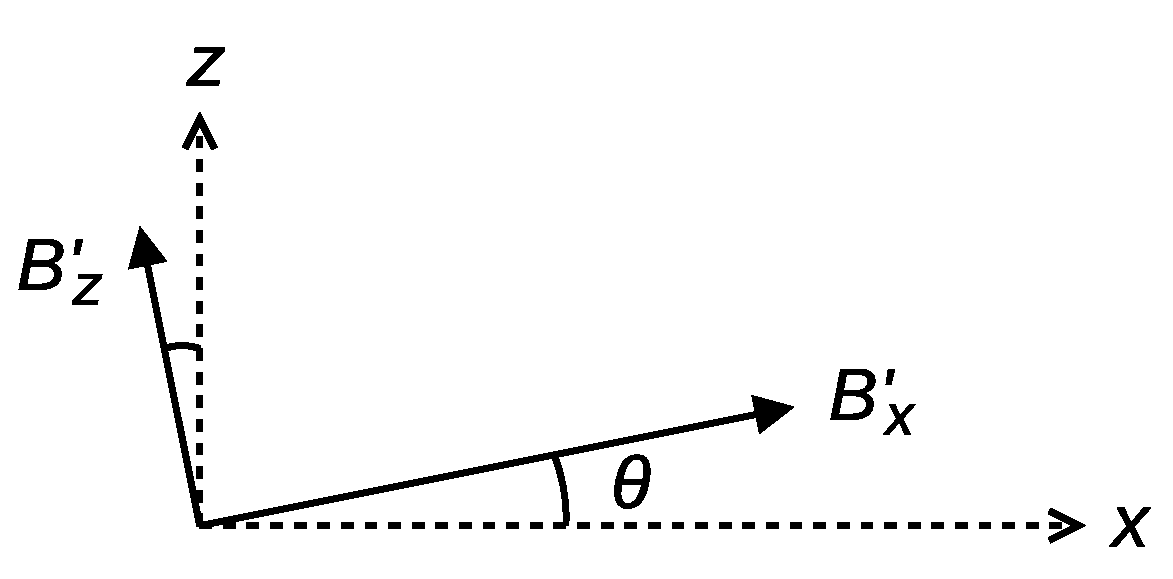
\includegraphics[width=0.45\textwidth]{figures/probe_tilt.eps}
\caption{\label{fig:angle} A diagram of the probe tilt. The $x$ and $z$ axes are correct relative
to the magnet. However, because the probe is tilted at some angle $\theta$, the given $B_x'$ and $B_z'$
are misaligned.}
\end{figure}

%Knowing $\theta$, we could find the correct $B_x$ and $B_z$:
%
%\begin{align*}
%B_x &= B'_x \cos\theta - B'_z \sin\theta \\
%B_z &= B_z' \cos\theta + B_x' \sin\theta
%\end{align*}
%
%To find $\theta$, we use the knowledge that $\theta$ is small and that, at magnet center,
%$B_z$ should be 0:
%
%\begin{align*}
%B_x &= B'_x - B'_z \theta \\ B_z &= B_z' + B_x' \theta \\
%\theta &= -\frac{B'_z}{B'_x}.
%\end{align*}

\subsection{Normalization}

Simulation output from \texttt{RotationShield} gives the magnetic field in arbitrary units, so the expected
magnetic field strength at any location is known only relative to another known location. To compare these simulations
with our measured output, we draw a small cube around magnet centerin the measured map,
calculate the average $B_x$ inside, and normalize the simulated map such that $B_x$ at its center matches the
measured map. This adjustment allows fair comparison of absolute field strengths at any location.

\subsection{Error bars}

The magnetic probe provides error bars for each measurement point. All error bars in plotted curves were found
to be below 0.2 mG, negligible in the following plots with ranges of 250 to 300 mG on the $y$-axis.

\section{Field profiles}

\subsection{Axial shield normal, endcap normal}

\begin{figure*}
    \includegraphics[width=\textwidth]{figures/normnorm_comp.eps}
    \caption{\label{fig:normnorm_comp}Comparison of simulated and measured $B_z$ vs. $z$ curves with
    both the axial shield and the endcap in a normal state.}
\end{figure*}

Before making predictions about the superconducting (SC) cases, comparing measurements with both lead components in
a normal state to corresponding simulations offers insight into the discrepancies between the simulated and real
systems. Initial versions of these comparisons reveal the need for the various aforementioned corrections.

Figure \ref{fig:normnorm_comp} shows simulated and measured $B_z$ vs. $z$ curves in the ``normal, normal'' case,
demonstrating good agreement with simulations.

\subsection{Axial shield superconducting, endcap normal}

\begin{figure*}
    \includegraphics[width=\textwidth]{figures/SCnorm_comp_new.eps}
    \caption{\label{fig:SCnorm_comp}Comparison of simulated and measured $B_z$ vs. $z$ curves with the
    axial shield superconducting, but the endcap in a normal state, overlaid with the simulated
    curve from Figure
     \ref{fig:normnorm_comp} to show agreement between the ``normal, normal'' and ``SC, normal'' cases.}
\end{figure*}

%By design, the axial shield is meant to protect the field from environmental influences, not to shape the field
%for better uniformity. Therefore,

Upon activating the axial shield by bringing it to superconducting (SC) temperature,
but leaving the endcap in a normal state, we expect minimal change in the field in the region that is being
plotted for two reasons. First, the Metglas shield (whose main purpose is to enforce field uniformity) is already
present, so the role of the axial shield is reduced. Second, by design, the axial lead shield has a greater effect on
the field at magnet center. This study, however, focuses on the field near the top endcap, away from magnet center.

Figure \ref{fig:SCnorm_comp}
shows the simulated and measured curves for the ``SC, normal'' as well as the
simulatede ``normal, normal'' curve
from Figure \ref{fig:normnorm_comp}. The simulated curves are almost indistinguishable,
showing the expectation that the effect of the axial shield should be negligible. This
expectation seems reasonable as the ``SC, normal'' measured curve shows minimal deviation from
the simulations.

\begin{figure*}
    \includegraphics[width=\textwidth]{figures/axial_effect.eps}
    \caption{\label{fig:SCnorm_hd}$B_z$ vs. $z$ as predicted by simulations with variations in the height
    of the axial shield. The cyan curve (no axial shield) and the magenta curve (axial shield height at
    1.100 m) are indistinguishable. Greater axial shield heights result in further suppression of the
    $B_z$ peak.}
\end{figure*}

It is interesting to note that, according to simulations, this is not always the case. Figure \ref{fig:SCnorm_hd}
shows simulated curves for the ``SC, normal'' configuration with 5 mm variations in the height of the axial shield,
along with a curve for the ``normal, normal'' configuration. When the axial shield's length is 1.100 m, the
``SC, normal'' curve seems indistinguishable from the ``normal, normal'' curve.
A similar variation, where the axial shield height was held constant and the height of the Metglas shield was varied,
yielded similar results. This suggests that the influence of the axial shield depends on the
height difference between it and the Metglas shield - the further the axial shield extends above the Metglas,
the more effectively it suppresses the $B_z$ peak.

\subsection{Axial shield superconducting, endcap superconducting}

\begin{figure*}
    \includegraphics[width=\textwidth]{figures/axial_effect_endcap.eps}
    \caption{\label{fig:SCSC_hd}$B_z$ vs. $z$ as predicted by simulations with the same variations in the height
    of the axial shield as in Figure \ref{fig:SCnorm_hd}, but with the superconducting endcap present. The
    suppression of the $B_z$ peak is no longer visible.}
\end{figure*}

Figure \ref{fig:SCSC_hd} shows the same axial shield height variation as in Figure \ref{fig:SCnorm_hd}, but with
the endcap included at a fixed height ($z = 1.128$ m) in each case, showing that the curves that were clearly
distinct without the endcap become harder to distinguish in the presence of the superconducting endcap.

\begin{figure*}
    \includegraphics[width=\textwidth]{figures/SCSC_comp.eps}
    \caption{\label{fig:SCSC_comp}Comparison of simulated and measured $B_z$ vs. $z$ curves with both the
    axial shield and the endcap in a superconducting state.}
\end{figure*}

In addition to the endcap's large-scale effects on field profiles, it is important to observe that its addition
should not significantly alter field gradients in the measurement cell volumes. Table \ref{tbl:gradients} shows
volume-averaged components of the gradient of $\vec{B}$ in the measurement cell calculated from high-resolution
simulations. These results suggest that we are justified in comparing field gradients with and without the endcap.

\begin{table*}
\begin{tabular}{R{2.8cm}|R{2.8cm}|R{2.8cm}|R{2.8cm}|R{2.8cm}}
    & \textbf{``norm, norm''} & \textbf{``SC, normal''} & \textbf{``SC, SC''} & \textbf{cap change}\\\hline
    \textbf{$\partial B_x/\partial x$} & -0.287690 & -0.285294 & -0.290683 & 0.005389 \\
    \textbf{$\partial B_y/\partial x$} & 0.000005 & -0.000020 & -0.000115 & 0.000095 \\
    \textbf{$\partial B_z/\partial x$} & -0.000001 & 0.003045 & 0.030903 & -0.027858 \\
    \textbf{$\partial B_x/\partial y$} & 0.000001 & 0.000011 & 0.000009 & 0.000002 \\
    \textbf{$\partial B_y/\partial y$} & 0.318764 & 0.317201 & 0.315975 & 0.001226 \\
    \textbf{$\partial B_z/\partial y$} & 0.000001 & 0.000002 & 0.000001 & 0.000001 \\
    \textbf{$\partial B_x/\partial z$} & 0.000000 & -0.018646 & -0.028932 & 0.010286 \\
    \textbf{$\partial B_y/\partial z$} & 0.000001 & -0.000002 & -0.000021 & 0.000019 \\
    \textbf{$\partial B_z/\partial z$} & -0.039736 & -0.041182 & -0.037189 & -0.003993 \\
\end{tabular}
\caption{\label{tbl:gradients} Simulated volume-averaged gradients in the measurement cell, in $\mu$G/cm, with a
central field of 30 mG. ``Cap change'' is the change due to the endcap when the axial shield is already SC.
Changes smaller than 0.1 $\mu$G/cm are negligible in measurement.}
\end{table*}

\section{Analysis}

Figures \ref{fig:normnorm_comp}, \ref{fig:SCnorm_comp}, and \ref{fig:SCSC_comp} all show good agreement between
measurement
and simulation. As expected, the endcap shifts the $B_z$ peak, a main source of non-uniformity, away
from magnet center. Comparisons show that our simulations are effective at predicting the endcap behavior, motivating
further simulated studies of different endcap geometries.

The study of simulations with varying axial shield heights (Figures \ref{fig:SCnorm_hd} and \ref{fig:SCSC_hd})
show that the expectation that the axial shield itself will not significantly alter the field only holds when
the Metglas-axial shield height difference is small. That the axial shield exertts a stronger influence on the interior
field when more of it is left ``uncovered'' by the Metglas shield is not surprising. However, Figure \ref{fig:SCSC_hd}
clearly shows that the introduction of the superconducting endcap effectively hides the axial shield's direct
influence on the field.

The tight agreement between the measured ``normal, normal'' and ``SC, normal'' cases seen in figure
\ref{fig:SCnorm_comp} indicates that, in our half-scale model, the Metglas-axial shield height difference is
indeed sufficiently small. Introducing the endcap in these simulatiosn suggests that, even if our estimate of
the Metglas-axial shield height difference is innacurate, the presence of the endcap could partially hide the effects
of that error.

Furthermore, gradient changes expected due to the endcap (see \ref{tbl:gradients}) are all well below 0.1 $\mu$G/cm,
which suggests that
good uniformity can be maintained with the endcap.

\section{Acknowledgments}

The author is grateful for support from the Arthur R. Adams SFP Fellowship.

\begin{thebibliography}{}
\bibitem{cpv} Cronin, J. ``Nobel Lecture: CP Symmetry Violation – The Search
for Its Origin,'' Nobel Media AB (2013).
\bibitem{ill} Baker, C. A., D. D. Doyle, P. Geltenbort, K. Green, M. G. D. Van der Grinten, P. G. Harris, P. Iaydjiev et al. ``Improved experimental limit on the electric dipole moment of the neutron.'' \textit{Physical Review Letters} 97, no. 13 (2006): 131801.
\bibitem{pendlebury} Pendlebury et. al. ``Geometric-phase-induced false electric dipole moment signals for particles in traps.'' \textit{Phys. Rev. A.} 70, 032102 (2004).
\bibitem{krl} ``Search for the nEDM at Caltech.'' Kellogg Radiation Laboratory
$\langle$krl.caltech.edu$\rangle$ (2014).
\bibitem{endcapstyles} Malkowski, S., R. Y. Adhikari, J. Boissevain, C. Daurer, B. W. Filippone, B. Hona, B. Plaster, D. Woods, and H. Yan. ``Overlap Technique for End-Cap Seals on Cylindrical Magnetic Shields.'' \textit{IEEE Transactions on Magnetics} 49, no. 1 (2013): 651-653.
\bibitem{coil} Perez Galvan, A., B. Plaster, J. Boissevain, R. Carr, B. W. Filippone, M. P. Mendenhall, R. Schmid, R. Alarcon, and S. Balascuta. ``High uniformity magnetic coil for search of neutron electric dipole moment.'' \textit{Nuclear Instruments and Methods in Physics Research Section A: Accelerators, Spectrometers, Detectors and Associated Equipment} 660, no. 1 (2011): 147-153.
\bibitem{rotshield} Mendenhall, M. P. \texttt{RotationShield} source. $\langle$https://github.com/mpmendenhall/rotationshield$\rangle$ (2014).
\end{thebibliography}

\end{document}
